

Due to the sensitivity of the beam coupling impedance to the boundary conditions of the equipment used, it is necessary to utilise different measurement techniques to fully analyse the impedance of accelerator structures.

\section{Low Q-factor Impedances}

For structures that are expected to contain mostly low Q-resonances (i.e. resistive wall impedance) it is appropriate to use the coaxial wire method[ref], sometimes also called the stretched wire method. This method relies on the similarity of the electromagetic field profile due to an ultrarelativistic charged particle and that of a short electrical pulse sent along a coaxial wire. 

An moving charged particle produces an electromagnetic field in a arc transverse to its direction of motion, where the angle of the arc opening is proportinal to the relativistic factor of the particle $\gamma$. For an ultrarelativistic particle ($\gamma \leftarrow \infty$), the field becomes entirely perpendicular to the direction of motion. If we place a conductive wire along the same path we would expect the charged particle to take (in most cases this is well represented by a straight wire), a short electrical pulse sent along this wire would propogate in the TEM (transverse electrical and magnetic field) mode, producing a field profile similar to that emitted by the ultrarelativistic charged particle (see. Fig. \ref{fig:coax-part-profile})


\begin{figure}

\caption{Comparison of the electromagnetic field profile of a moving charged particle and a short time pulse propogating along a coaxial wire.}
\label{fig:coax-part-profile}
\end{figure}

\subsection{Classical Coaxial Wire Method}

The classical coaxial wire method, first proposed by V. Vaccarro in 1990 [ref], is a transmission method that measures the complex transmission coefficient of a DUT (Device Under Test) made up of the equipment whose impedance is to be measured and a coaxial wire passing through it. 

The experimental setup is as shown in Fig. \ref{fig:classic-coax}. Firstly the external circuit (i.e. everything not the DUT) is matched to the characteristic impedance of the coaxial line inside the DUT. This is done by measuring the reflection coefficient $\Gamma$ for the setup with only one port connected to the DUT and the other end terminated by an open connection. Knowing the characteristic impedance of the VNA and associated cables (typically $Z_{0} = 50\Omega$), we can easily calculate the characteristic impedance, $Z_{c}$, from the relation,

\begin{equation}
\Gamma = \frac{Z_{c} - Z_{0}}{Z_{c} + Z_{0}}.
\end{equation}

We then electrically match the characteristic impedance by adding resistors in series just before the DUT to resistively match the characteristic impedance of the VNA to that of the DUT. It is possible to use physical matching also using transition cones but these are costly, time consuming to construct and require new cones for each piecof equipment measured. And as can be seen in Fig. \ref{fig:matching-plot}, matching with a resistor is highly effective at removing the presence of reflections in coaxial measurements.

\begin{figure}

\caption{Experimental setup for a measurement of the beam coupling impedance using the classical coaxial wire method}
\label{fig:classic-coax}
\end{figure} 

\begin{figure}

\caption{An example of a reflection measurement made with and without a matching resistor. The faded line is the measurement without matching, the bold line that with. The reduction in the reflection can be seen.}
\label{fig:matching-plot}
\end{figure}

The value that we wish to measure to evaluate the beam coupling impedance of a device are the scattering parameters of the resulting circuit, in particular $S_{21}$, the normalised transmission parameter through the DUT. $S_{21}$ is calculated by taking the measured transmission parameter $S_{21,DUT}$ and dividing it by the transmission parameter through a reference line of the same physical length as the DUT,

\begin{equation}
S_{21} = \frac{S_{21,DUT}}{S_{21,REF}}
\end{equation}.

The effect of this is to correct the measured phase change in the DUT to be that only caused by the imaginary component of the beam coupling impedance.

There are subsequently a number of ways to evaluate the beam coupling impedance of the DUT depending on it's expected properties. For devices that are expected to have a either a small impedance, or those that are physically very short in length, it is possible to use the so called lumped impedance formula[ref];

\begin{equation}
Z = 2Z_{c} \frac{1-S_{21}}{S_{21}}
\end{equation}.

For distributed impedances, it is suitable to use the so called log formula (called so due to attenuation causing a log function to appear in the evaluation),

\begin{equation}
Z = -2Z_{c} ln \left( S_{21} \right)
\end{equation}.

For long components or measurements at very high frequencies there exists the improved log formula. This takes into account more completely the electrical length of the device, given by

\begin{equation}
Z = -2Z_{c} ln \left( S_{21}  \right) \left( 1 + j\frac{ln \left( S_{21}\right) }{2\Theta}  \right)
\end{equation}

where $\Theta = 2\pi \frac{L}{\lambda}$ is the normalised electrical length of the device, $L$ the length of the device, $\lambda$ the wavelength of the frequency of measurement. It is possible to see that the lumped impedance formula can be used when $\Theta \leq 1$, and the improved log formula becomes useful for $\Theta \geq 5$[erk's paper].




\subsection{Resonator Coaxial Wire Method}

An alternative method for measuring the beam coupling impedance is by using the so called resonator method. The setup for this method is similar to that of the classical coaxial wire method, except that the matching resistor network between the VNA and DUT is replaced by a weak capacitive coupling ($S_{11} < 0.5dB$) at both ends of the DUT. This then produces a structure which resonates at frequencies where the wavelength corresponds to the classical closed structure form,

\begin{equation}
\lambda = \frac{2L}{n}
\end{equation}

where $\lambda$ is the wavelength of the resonance, n the harmonic of the resonance and L the length of the device. 

The resonant method enables accurate measurement of the transmission losses due to the real longitudinal impedance. Additional advantages are that no matching is required, and a large number of mechanical uncertainties (electrical connections, consistency of calibration) can be avoided. However it can be seen that the frequency resolution is limited due to the length of the DUT so the method is not recommended as the only measurement method for structures expected to contain high-Q, narrowband resonances. It can however be used to corroborate the results obtained using the classical method.

For each resonancce peak, the loaded Q-factor and the frequency of the resonance are measured. For a weak coupling at both ends of the DUT, we can write the coupling coefficient k as

\begin{equation}
k = \frac{\left| S_{21} \right|}{1 - \left| S_{21} \right| }.
\label{eqn:coupling_coeff}
\end{equation}

The difference between the unloaded $Q$-factor, $Q_{0}$ , and the loaded $Q$-factor, $Q_{L}$, is a function of k. We can get an approximate correction by using the formula

\begin{equation}
Q_{0} = Q_{L} \left( 1 + k  \right).
\label{eqn:Q_correc}
\end{equation}

Subsequently the measured line attenuation (in Np/m) is then calculated

\begin{equation}
\alpha_{m} = \frac{\pi}{\lambda Q_{0}}.
\label{eqn:atten}
\end{equation}

Note that this attenuation includes both that from the beam coupling impedance due to the finite resistance of the wire material. We can estimate the attenuation due to the wire material as

\begin{equation}
\alpha_{w} = \sqrt{\pi \rho_{w} \epsilon f} \frac{1}{d ln D/d}
\label{eqn:wire_atten}
\end{equation}

where $\rho_{w}$ is the wire resistivity, $\epsilon$ the permitivitty, $f$ the frequency, $d$ the diameter of the inner conductor and $D$ the diameter of the outer conductor. At very low frequencies the finite skin depth of the inner conductor would also have to be taken into account. Using the corrected attentuation $\alpha = \alpha_{m} - \alpha_{w}$, the real longitudinal impedance per unit length can be found to be 

\begin{equation}
\Re e\left\{ Z \right\} = 2Z_{c} \alpha
\label{eqn:res_imp}
\end{equation}

\begin{figure}

\label{fig:res-resonancce-examples}
\caption{An example of the resonance pattern seen whilst performing measurements using the resonant method. Each peak corresponds to one data point in the final measurements.}
\end{figure}

To calculate the imaginary impedance using the resonant method involves a more involved calculation. In particular it is necessary to carry out measurements using the resonant method on a reference pipe of the same physical length to the DUT, either using physical measurements or a simulated measurement.

If we consider the complex impedance of the two measurements, $Z_{DUT}$ for the DUT and $Z_{REF}$ for a perfectly conducting reference pipe, we can simplify them as

\begin{align}
Z_{DUT} & =  R + jX_{1}  =  Z_{1}e^{j \phi} \\
Z_{REF} & =  jX_{2}  =  Z_{2}e^{j.0}
\end{align}

where $R$ is the resistive component of the DUT impedance, $X_{1/2}$ the imaginary component of the impedance (DUT and reference pipe respectively), $\phi$ is the angle of DUT impedance projected onto a complex plane and $Z_{2} = \sqrt{R^{2} + X^{2}}$. If we consider a measured value depedent on the impedance, for example the transmission parameter $S_{21}$ at a resonance peak, we have the following relations

\begin{align}
S_{21}^{DUT} = S_{0}e^{j \left( \omega_{1}t + \phi \right)} \\
S_{21}^{REF} = S_{0}e^{k \left( \omega_{2}t \right)}
\end{align}

where $S_{0}$ is some normalised scalar, $\omega_{1/2}$ is the frequency of the resonance and $t = \frac{L}{c}$ . Thus for a pair of corresponding peaks from resonance measurements for which we have measured $\omega_{1}$ and $\omega_{2}$ we can equate $S_{21}^{DUT} = S_{21}^{REF}$ and thus show

\begin{equation}
\phi = t \left( \omega_{2} - \omega_{1} \right).
\end{equation}

Subsequently we can see that

\begin{equation}
X = Z_{DUT} sin \phi = R \frac {sin \phi}{cos \phi} = R tan \phi
\end{equation}

where $R = \Re e(Z)$.

\subsection{Transverse Impedance Measurements}

The above methods give a general impression of how to carry out coaxial wire measurements of the impedance of accelerator components. Directly applied as described they allow the measurement of the longitudinal impedance of a DUT. However, from a beam stability point of view it is often more interesting to look at the transverse imedance of a device. In particular it would be useful to have a method of determining the vertical/horizontal dipolar (or driving) impedance and the vertical/horizontal quadrupolar (detuning) impedance of any device. In this section we describe how do this for structures with top/bottom, left/right symmetry and then generalising to asymmetric structures, with illustration from simple examples evaluated using simulations.

To allow a complete explanation of how to verify the methods of measuring transverse impedances, let us first consider the general form of the $m$-th order ($m = 0, 1, 2,...$) longitudinal beam coupling impedance, given by [ref]

\begin{equation}
\bar{Z}_{m} = \frac{-1}{I^{2}} \int dV \mathbf{\bar{E}_{m}. \bar{J}_{m}^{*}}
\end{equation}

where $\bar{J}_{m}$ is the current density of the source. For a beam propogating along the z-axis with an offset a and moment $cos \left( m \theta \right)$,

\begin{equation}
\mathbf{\bar{J}_{m}} = \frac{I}{\pi a^{m +1} \left( 1 + \delta_{m0} \right)} \delta \left( r - a \right) cos \left( m \theta \right) exp \left( j \left( \omega t - k z  \right) \right) \mathbf{e_{z}}.
\end{equation}

The electromagnetic field associated with a given current source $\mathbf{\bar{J}_{m}}$ is $\left( \mathbf{\bar{E}_{m}}, \mathbf{\bar{H}_{m}} \right)$. 

What can be seen is that any different azimuthal components of the $m$-th field of order n (i.e. $sin \left( n\theta \right)$ and $cos \left( n\theta \right)$ terms) are neglected in this treatment. To allow the treatment of coupling between different azimuthal orders we can define a longitudinal beam coupling impedance $Z_{m,n}$ (where $m,n = 0, \pm 1, \pm 2, ... $)

\begin{equation}
Z_{m,n} = \frac{-1}{I^{2}} \int dV \mathbf{E_{m}. J_{n}^{*}}
\end{equation}

where

\begin{equation}
\mathbf{J_{m}} = \frac{I}{\pi a^{|m |+1}} \delta \left( r - a \right) exp \left(j m \theta \right) exp \left( j \left( \omega t - k z  \right) \right) \mathbf{e_{z}}.
\end{equation}

Importantly, this allows us to see that 

\begin{align}
\mathbf{\bar{J}_{0}} &= \mathbf{J_{0}} \nonumber \\
\mathbf{\bar{J}_{m}} &= \mathbf{J_{m}} + \mathbf{J_{-m}}.
\end{align}

From here we use the principle of superposition for electromagnetic fields, and thus can derive

\begin{align}
\bar{Z}_{0} &= Z_{0} \\
\bar{Z}_{x} &= \bar{Z}_{1} = Z_{1,1} + Z_{1,-1} + Z_{-1,1} + Z_{-1,-1} = kZ^{dip}_{x}\\
\bar{Z}_{x} &= \bar{Z}_{1} \text{(cos replaced with sin)}= Z_{1,1} - Z_{1,-1} - Z_{-1,1} + Z_{-1,-1} = kZ^{dip}_{y}\\
\bar{Z}_{m} &= Z_{m,m} + Z_{m,-m} + Z_{-m,m} + Z_{-m,-m}, m=1,2,...
\end{align}

From this start we will apply this two both two wire measurements and to displaced single wire measurements.

\subsubsection{Two Wire Measurements}

It is possible to directly measure the dipolar impedance of a device through the use of a two wire coaxial method. The measurement setup is identical to that of the single wire method, except that two wires, seperated by distance $\Delta$, are placed in the device, and a 180$^{\circ}$ hybrid is place between the wires and the VNA at both ends of the device. This setup is illustrated in Fig. \ref{fig:two_wire_measure}

\begin{figure}

\label{fig:twowiremeasure}
\caption{Measurement setup for measurements of the dipolar beam coupling impedance using the two wire setup for the classical coaxial wire method.}
\end{figure}

The measurements are done in the same way as described in the previous sections for either the classical transmission method or the resonator method. By using two wires each carrying a signal 180$^{o}$ out of phase with one another we produce a field pattern similar to a dipole and thus measure the dipole impedance in either the horizontal or vertical plane depending on the orientation of the two wires. 

What is directly measured is the longitudinal impedance of just the dipole impedance, as is to be expected from the Panofsky-Wenzel theorem (see Chap. \ref{chap:wake_imp} for further explanation). 

For two wire placed as positions $x = \pm a$, the current density is given by [ref]

\begin{align}
J & =  I \left( \delta \left( x - a \right) - \delta \left( x + a  \right) \right) \delta (y) exp \left( j \left( \omega t - kz \right) \right) \nonumber \\
& =  \frac{I}{\pi a} \displaystyle\sum\limits_{m=-\infty}^{\infty} exp \left(j \left( 2m +1 \right) \theta \right) exp \left( j \left( \omega t - kz \right) \right) \nonumber \\
& =  2\displaystyle\sum\limits_{m=-\infty}^{\infty} a^{|2m + 1 |} J_{2m + 1}.
\end{align}

The impedance is then

\begin{align}
Z & =  - \frac{1}{I^{2}} \int dV \left( 2\displaystyle\sum\limits_{m=-\infty}^{\infty} a^{|2m + 1 |} E_{2m + 1}  \right)  \left( 2\displaystyle\sum\limits_{n=-\infty}^{\infty} a^{|2n + 1 |} J_{2n + 1}^{*}  \right) \nonumber \\
& =  4 \displaystyle\sum\limits_{m,n} a^{|2m + 1 | + |2n + 1|} Z_{2m + 1, 2n+1} \nonumber \\
& =  \left(2a \right)^{2}\left( Z_{1,1} + Z_{-1,1} + Z_{1,-1} + Z_{-1,-1} \right) + O(a^{4}) \nonumber \\
& =  (2a)^{2}\bar{Z}_{x} + O(a^{4}). 
\end{align}

Again using the Panofsky-Wenzel theorem we can deduce that the transverse dipolar impedance $Z^{dip}_{x/y}$ is given by 

\begin{equation}
Z^{dip}_{x/y} = \frac{\bar{Z}_{x/y}}{k} = \frac{c}{\omega} \frac{Z}{\Delta^{2}}
\end{equation}

where $\Delta = 2a$ and $Z$ is the measured complex impedance.

\subsubsection{Structures with Top/Bottom, Left/Right Symmetry}

If we consider a source particle at at $x_{1} = a_{1}cos\theta_{1}, y_{1} = a_{1}sin\theta_{1}$ and a test particle at $x_{2} = a_{2}cos\theta_{2}, y_{2} = a_{2}sin\theta_{2}$, the source current density is

\begin{align}
J_{z} &= I\delta \left( x-x_{1} \right) \delta \left( y-y_{1} \right) exp \left( k \left( \omega t - kz \right) \right) \nonumber \\
          &=\displaystyle\sum\limits_{m=-\infty}^{\infty}a_{1}^{|m|}exp\left( -jm\theta_{1} \right) J_{m}
\end{align}

The impedance would therefore be

\begin{align}
Z = &\frac{-1}{I^{2}} \int dV \left( \displaystyle\sum\limits^{\infty}_{m=-\infty} a_{1}^{|m|} exp \left( jm\theta_{1} \right) E_{m}\right) \left( \displaystyle\sum\limits^{\infty}_{n=-\infty} a_{1}^{|n|} exp \left( jn\theta_{2} \right) J^{*}_{n}\right) \nonumber \\
   = &\displaystyle\sum\limits^{\infty}_{m,n=-\infty} a_{1}^{|m|} a_{2}^{|n|} exp\left( -jm\theta_{1} \right) exp\left( -jn\theta_{2} \right) Z_{m,n} \nonumber \\
   = &Z_{0,0} + \left( x_{1}- jy_{1} \right)Z_{1,0} + \left( x_{1} + jy_{1} \right)Z_{-1,0} + \left( x_{2} + jy_{2} \right)Z_{0,1} +  \left( x_{2} - jy_{2} \right)Z_{0,-1} \nonumber \\
      & +\left( x_{1} - jy_{1} \right)^{2}Z_{2,0} +  \left( x_{1} - jy_{1} \right)\left( x_{2} - jy_{2} \right)Z_{1,-1} + \left( x_{2} - jy_{2} \right) Z_{0,-2} \nonumber \\
      & +\left( x_{1} - jy_{1} \right)\left( x_{2} + jy_{2} \right)Z_{1,1} + \left( x_{1} + jy_{1} \right) \left( x_{2} - jy_{2} \right) Z_{-1,-1} \nonumber \\
      & +\left( x_{1} + jy_{1} \right)^{2}Z_{-2,0} + \left( x_{1} + jy_{1} \right)\left( x_{2} - jy_{2} \right) Z_{-1,1} + \left( x_{2} - jy_{2} \right)^{2}Z_{0,2} \nonumber \\
      & +O\left( \left(  x_{1},y_{1},x_{2},y_{2} \right)^{3} \right).
\label{eqn:gen_imp}
\end{align}

By applying Panofsky-Wenzel we see

\begin{align}
kZ_{x} =\frac{\partial Z}{\partial x_{2}} = & Z_{0,1} + Z_{0,-1} + \left( x_{1} - jy_{1} \right) Z_{1,-1} + 2\left( x_{2} - jy_{2} \right) Z_{0,-2} \nonumber \\
						&+ \left( x_{1} - jy_{1} \right) Z_{1,1} + \left( x_{1} + jy_{1} \right) Z_{-1,-1} + \left( x_{1} + jy_{1} \right) Z_{-1,1} + 2\left( x_{2} + jy_{2} \right) Z_{0,2} \nonumber \\
						& + O\left( \left( x_{1},y_{1},x_{2},y_{2} \right)^{2} \right) \nonumber \\
						= & Z_{0,1} + Z_{0,-1} + x_{1}\bar{Z}_{x} + jy_{1} \left( -Z_{1,-1} - Z_{1,1} + Z_{-1,-1} + Z_{-1,1} \right) \nonumber \\
						& + x_{2}\left( 2Z_{0,-2} + 2Z_{0,2}  \right) + jy_{2}\left( -2Z_{0,-2} + 2Z_{0,2}  \right) +  O\left( \left( x_{1},y_{1},x_{2},y_{2} \right)^{2} \right)
\end{align}

\begin{align}
kZ_{y} =\frac{\partial Z}{\partial y_{2}} = & jZ_{0,1} - jZ_{0,-1} - j\left( x_{1} - jy_{1} \right) Z_{1,-1} - 2j\left( x_{2} - jy_{2} \right) Z_{0,-2} \nonumber \\
						&+ j\left( x_{1} - jy_{1} \right) Z_{1,1} - j\left( x_{1} + jy_{1} \right) Z_{-1,-1} + j\left( x_{1} + jy_{1} \right) Z_{-1,1} + 2j\left( x_{2} + jy_{2} \right) Z_{0,2} \nonumber \\
						& + O\left( \left( x_{1},y_{1},x_{2},y_{2} \right)^{2} \right) \nonumber \\
						= & j\left(Z_{0,1} - Z_{0,-1} \right)+ y_{1}\bar{Z}_{y} + jx_{1} \left( -Z_{1,-1} + Z_{1,1} + Z_{-1,-1} + Z_{-1,1} \right) \nonumber \\
						& + y_{2}\left(- 2Z_{0,-2} - 2Z_{0,2}  \right) + jx_{2}\left( -2Z_{0,-2} + 2Z_{0,2}  \right) +  O\left( \left( x_{1},y_{1},x_{2},y_{2} \right)^{2} \right).
\end{align}

Two properties to note for later use are that

\begin{align}
\textbf{J}_{-m} \left( \omega \right) & = \textbf{J}_{m}^{*} \left( -\omega \right) \\
Z_{-m,-n} \left( \omega \right) & = Z_{m,n}^{*} \left( -\omega \right).
\end{align}

If we now assume a single wire rather than a source and test particle, such that $x_{1}=x_{2}=x_{0}, y_{1}=y_{2}=y_{0}$. This gives a source current density

\begin{align}
J & = I \delta \left( x-x_{0} \right)\delta \left( y-y_{0} \right) exp\left( j \left(\omega t -kz \right)\right) \nonumber \\
  & = \frac{I}{2\pi a} \delta \left( r-a \right)\displaystyle\sum\limits_{m=-\infty}^{\infty} exp\left( jm \left( \theta -\theta_{0} \right) \right) exp\left( jm \left( \theta -\theta_{0} \right) \right) exp\left( j \left( \omega t - kz \right) \right) \nonumber \\
  & = \displaystyle\sum\limits_{m=-\infty}^{\infty} a^{|m|}exp\left( -jm\theta_{0} \right)J_{m}.
\end{align}

We can then define $x_{0}=acos\theta_{0}, y_{0}=asin\theta_{0}$. Entering this into Eqn. \ref{eqn:gen_imp} gives

\begin{align}
Z &=&Z_{0,0} +  \left( x_{0} - jy_{0} \right) Z_{1,0} + \left( x_{0} + jy_{0} \right)  Z_{-1,0} + \left( x_{0} + jy_{0} \right) Z_{0,1} \nonumber \\
   &   &+ \left( x_{0} - jy_{0} \right) Z_{0,-1} + \left( x_{0} - jy_{0} \right)^{2} Z_{2,0} + \left( x_{0} - jy_{0} \right)^{2} Z_{1,-1} + \left( x_{0} - jy_{0} \right) ^{2}Z_{0,-2} \nonumber \\
   &   &+\left( x_{0} - jy_{0} \right) \left( x_{0} + jy_{0} \right) Z_{1,1} + \left( x_{0} + jy_{0} \right)\left( x_{0} - jy_{0} \right) Z_{-1,-1} + \left( x_{0} + jy_{0} \right)^{2}Z_{-2,0} \nonumber \\
   &   &+\left( x_{0} + jy_{0} \right)^{2} Z_{-1,1} + \left( x_{0} + jy_{0} \right)^{2}Z_{0,2} + O\left( \left(x_{0},y_{0} \right)^{2} \right) \nonumber \\
   &=&Z_{0,0} + x_{0}\left( Z_{1,0}+Z_{-1,0}+Z_{0,1}+Z_{0,-1} \right) +jy_{0} \left( -Z_{-1,0} + Z_{-1,0} + Z_{0,1} - Z_{0,-1} \right) \nonumber \\
   &   &+x_{0}^{2} \left(  Z_{1,-1}+Z_{1,1}+Z_{-1,-1}+Z_{-1,1} + Z_{2,0} + Z_{0,-2} + Z_{0,2} + Z_{-2,0} \right) \nonumber \\
   &   &+y_{0}^{2} \left(  -Z_{1,-1}+Z_{1,1}+Z_{-1,-1}-Z_{-1,1} - Z_{2,0} - Z_{0,-2} - Z_{0,2} - Z_{-2,0} \right) \nonumber \\
   &   &+2jx_{0}y_{0}\left( -Z_{2,0} - Z_{0,-2} + Z_{-2,0} + Z_{0,2} + Z_{-1,1} - Z_{1,-1} \right) \nonumber \\
   &=&Z_{0,0} + x_{0}\left( Z_{1,0}+Z_{-1,0}+Z_{0,1}+Z_{0,-1} \right) +jy_{0} \left( -Z_{-1,0} + Z_{-1,0} + Z_{0,1} - Z_{0,-1} \right) \nonumber \\
   &   &+x_{0}^{2} \left( \bar{Z}_{x} + Z_{2,0} + Z_{0,-2} + Z_{0,2} + Z_{-2,0} \right) \nonumber \\
   &   &+y_{0}^{2} \left( \bar{Z}_{y} - Z_{2,0} - Z_{0,-2} - Z_{0,2} - Z_{-2,0} \right) \nonumber \\
   &   &+2jx_{0}y_{0}\left( -Z_{2,0} - Z_{0,-2} + Z_{-2,0} + Z_{0,2} + Z_{-1,1} - Z_{1,-1} \right).
\label{eqn:gen_single_wire}
\end{align}

It can then be seen that if measurements are made with $x_{0} = 0$ and take different values of $y_{0}$ that one obtains data with a parabolic fit in the $y_{0}$ axis. Be fitting a curve to this we obtain constant (equal to the longitudinal impedance), linear and quadratic terms. Doing the same for $y_{0}=0$ allows us to derive two quadratic terms

\begin{align}
Z^{\perp}_{x} & = \left( \bar{Z}_{x} + kZ_{quad} \right)\frac{1}{k} =  Z^{dip}_{x} + kZ_{quad}\\
Z^{\perp}_{y} & = \left( \bar{Z}_{y} - kZ_{quad} \right)\frac{1}{k}= Z^{dip}_{y} - kZ_{quad} \\
\end{align}

where $Z_{quad}=\frac{1}{k}\left( Z_{0,2}+Z_{2,0}+Z_{0,-2}+Z_{-2,0}  \right) = \frac{2}{k}\left( Z_{0,2}+Z_{0,-2}  \right)$, representing the impedance due to the displacement of the test particle in an accelerator. As we can measure $\bar{Z}_{x/y}$ independently using the two wire method we can thus indepedently measure $Z_{quad}$ using a displaced single wire scan in both the x- and y-planes.

It can also be seen that

\begin{align}
Z^{\perp}_{x} + Z^{\perp}_{y} = \frac{1}{k}\left( \bar{Z}_{x} + \bar{Z}_{y} \right) = Z^{dip}_{x} + Z^{dip}_{y}
\end{align}

where $\bar{Z}_{x/y}$ can be measured independently which gives a method of obtaining confidence in the wire measurements.

\subsubsection{Asymmetric Structures}

If Eqn. \ref{eqn:gen_single_wire} is transformed from $\left( x,y \right)$ coordinates to $\left( a, \theta \right)$, the result is

\begin{align}
Z &=Z_{0,0} +a\left[ cos\theta \left( Z_{-1,0} + Z_{0,1} \right) +jsin\theta \left( Z_{-1,0} + Z_{0,1} \right)  cos\theta \left( Z_{1,0} + Z_{0,-1} \right) - jsin\theta \left( Z_{1,0} + Z_{0,-1} \right)\right] \nonumber \\
   &+a^{2}\left[ cos^{2} \left( Z_{1,1} + Z_{-1,-1} \right) + sin^{2} \left( Z_{1,1} + Z_{-1,-1} \right)\right] \nonumber \\
   &+a^{2}\left[ cos^{2} \left( Z_{2,0} + Z_{0,-2} +Z_{1,-1} \right) +2jsin\theta cos\theta\left( Z_{2,0} + Z_{0,-2} +Z_{1,-1} \right) \right] \nonumber \\
   & - a^{2}\left[sin^{2} \left( Z_{2,0} + Z_{0,-2} +Z_{1,-1} \right)\right] \nonumber  \\
   &+ a^{2}\left[ cos^{2} \left( Z_{-2,0} + Z_{0,2} +Z_{-1,1} \right) +2jsin\theta cos\theta\left( Z_{-2,0} + Z_{0,2} +Z_{-1,1}  \right) \right] \nonumber \\
   &+ a^{2}\left[sin^{2} \left( Z_{-2,0} + Z_{0,2} +Z_{-1,1}  \right) \right].
\end{align}

Grouping like terms this becomes
\begin{align}
Z   &=Z_{0,0} + a\left[ e^{-j\theta}\left( Z_{-1,0} + Z_{0,1} \right) +  e^{j\theta}\left( Z_{1,0} + Z_{-0,1} \right)\right] \nonumber \\
     &+a^{2}\left[ \left( Z_{1,1} + Z_{-1,-1} \right) + e^{-2j\theta} \left(  Z_{2,0} + Z_{0,-2} +Z_{1,-1} \right) + e^{2j\theta} \left( Z_{-2,0} + Z_{0,2} +Z_{-1,1} \right) \right] \nonumber \\
     &=A_{1} + ae^{-j\theta}A_{2} + ae^{-j\theta}A_{3}+ a^{2}e^{-2j\theta}A_{4} +a^{2}e^{2j\theta}A_{5} +  a^{2}A_{6}
\label{eqn:rot_gen}
\end{align}

where $A_{1} = Z_{0,0}$, $A_{2} = Z_{0,1}+Z_{-1,0}$, $A_{3} = Z_{0,-1}+Z_{1,0}$, $A_{4} = Z_{0,2}+Z_{-1,1}+Z_{-2,0}$, $A_{5} = Z_{2,0}+Z_{1,-1}+Z_{0,-2}$ and $A_{6}=Z_{1,1}+Z_{-1,-1}$. Taking the earlier definition of $Z_{quad}$ it can be deduced that

\begin{align}
Z_{quad} & = \left( A_{4}+A_{5}+A_{6} - \bar{Z}_{x} \right)\frac{1}{k} =\frac{ A_{4}+A_{5}+A_{6}}{k} - Z^{dip}_{x} \\  
	    & = \left( A_{4}+A_{5} - \frac{\bar{Z}_{x}- \bar{Z}_{y}}{2}\right)\frac{1}{k} =\frac{ A_{4}+A_{5}}{k} - \frac{Z^{dip}_{x}-Z^{dip}_{y} }{2}.
\end{align}

Consideration of Eqn. \ref{eqn:rot_gen} lets it be seen that

\begin{align}
 A_{4}+A_{5}+A_{6} & = \frac{Z\left( a,0 \right)+Z\left( a,\pi \right) - 2Z\left( 0,0 \right)}{2a^{2}} \\
 A_{4}+A_{5} & = \frac{Z\left( a,0 \right)+Z\left( a,\pi \right) - Z\left( a,\frac{\pi}{2} \right)-Z\left( a,\frac{3\pi}{2} \right)}{2a^{2}}
\end{align} 

\subsection{Measurements on Example Geometries}

In this section shall be presented a number of example analyses of coaxial wire measurements done on geometries exhibiting top/bottom, left/right symmetry and an asymmetric structure. This permits a step-by-step guide to analysis of the wire measurements, which may not be immediately clear from the mathematical introduction. These simulations are simulated using both Ansoft HFSS and Maxwell using a driven modal solution. The measurement system is simulated by placing waveguide ports at either end of the geometry with a conducting cylinder placed as the inner conductor of the coaxial system. The transmission parameters are then acquired 

\subsubsection{Structure with Top/Bottom, Left/Rght Symmetry}

For the structure exhibiting top/bottom, left/right symmetry we use the Tsutsui model of two parallel plates as shown in Fig.~\ref{fg:tsutsui-model}. We use this due to the model allowing the prediction of the longitudinal, dipolar and quadrupolar impedances for a wide variety of materials and frequency ranges [cite Tsutsui longitudinal, transverse]. 


\begin{figure}
\subfigure[]{
\label{fig:tsutsui-model}
}

\subfigure[]{

\label{fig:zannini-model}
}
\label{fig:wire-measure-geometries}
\caption{The geometries used for coaxial wire measurement simulations. For the geometry with top/bottom, left/right symmetry we use the Tsutsui model (\ref{fig:tsutsui-model}) using two parallel plates. For the asymmetric structure we use the Zannini-model for a c-core ferrite kicker magnet (\ref{fig:zannini-model}), which generates a constant term and a noticeable asymmetric term.}
\end{figure}

\section{High Q-factor Impedances}

For high Q-factor impedances, such as cavity impedances, it is not appropriate to use a coaxial wire method to measure the impedance due to the large perturbation of the boundary conditions that it causes [ref Vaccaro coaxial method], in particular below the cut-off frequency of the connecting beam pipes. This is due to the presence of the coaxial wire reducing the cut-off frequency to 0Hz, thus allowing propogation losses at all frequencies rather than just above cut-off. To illustrate this, we can consider the total Q of a cavity to be related to the "trapped" cavity mode Q and the propogation losses as;

\begin{equation}
\frac{1}{Q_{total}} = \frac{1}{Q_{cavity}} + \frac{1}{Q_{prop}}
\end{equation}

Under excitation by a charged particle beam, propogation losses do not exist below the cutoff frequency and thus $Q_{prop} = 0$. However, the addition of the coaxial wire causes these propogation losses to occur at all frequencies. Importantly, the Q-factor of these propogation losses is of a similar magnitude or smaller than that of the cavity resonance, leading to a great distortion of the measured Q. Similarly, the perturbation of the conductive wire in the centre of the structure leads to a shift in the resonance frequency of the cavity modes. 

To illustrate this phenomena, a number of simulations have been carried out to compare the measurements using the coaxial wire method compared to the impedance as simulated using CST Particle Studio[ref]

\begin{figure}
\subfigure[]{
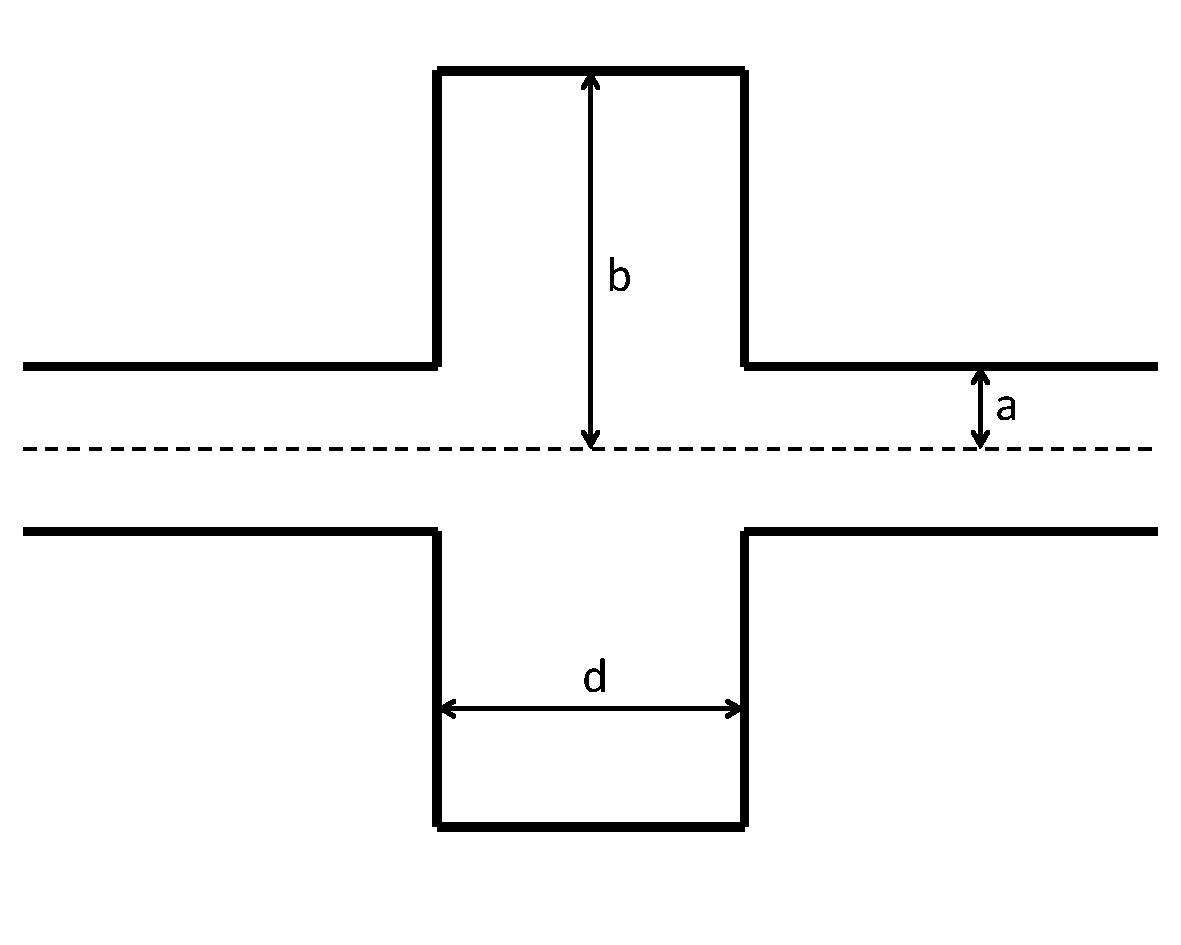
\includegraphics[width=0.5\linewidth]{figures/cavity_beampipe.pdf}
\label{fig:cavity_beampipe}
}
\subfigure[]{
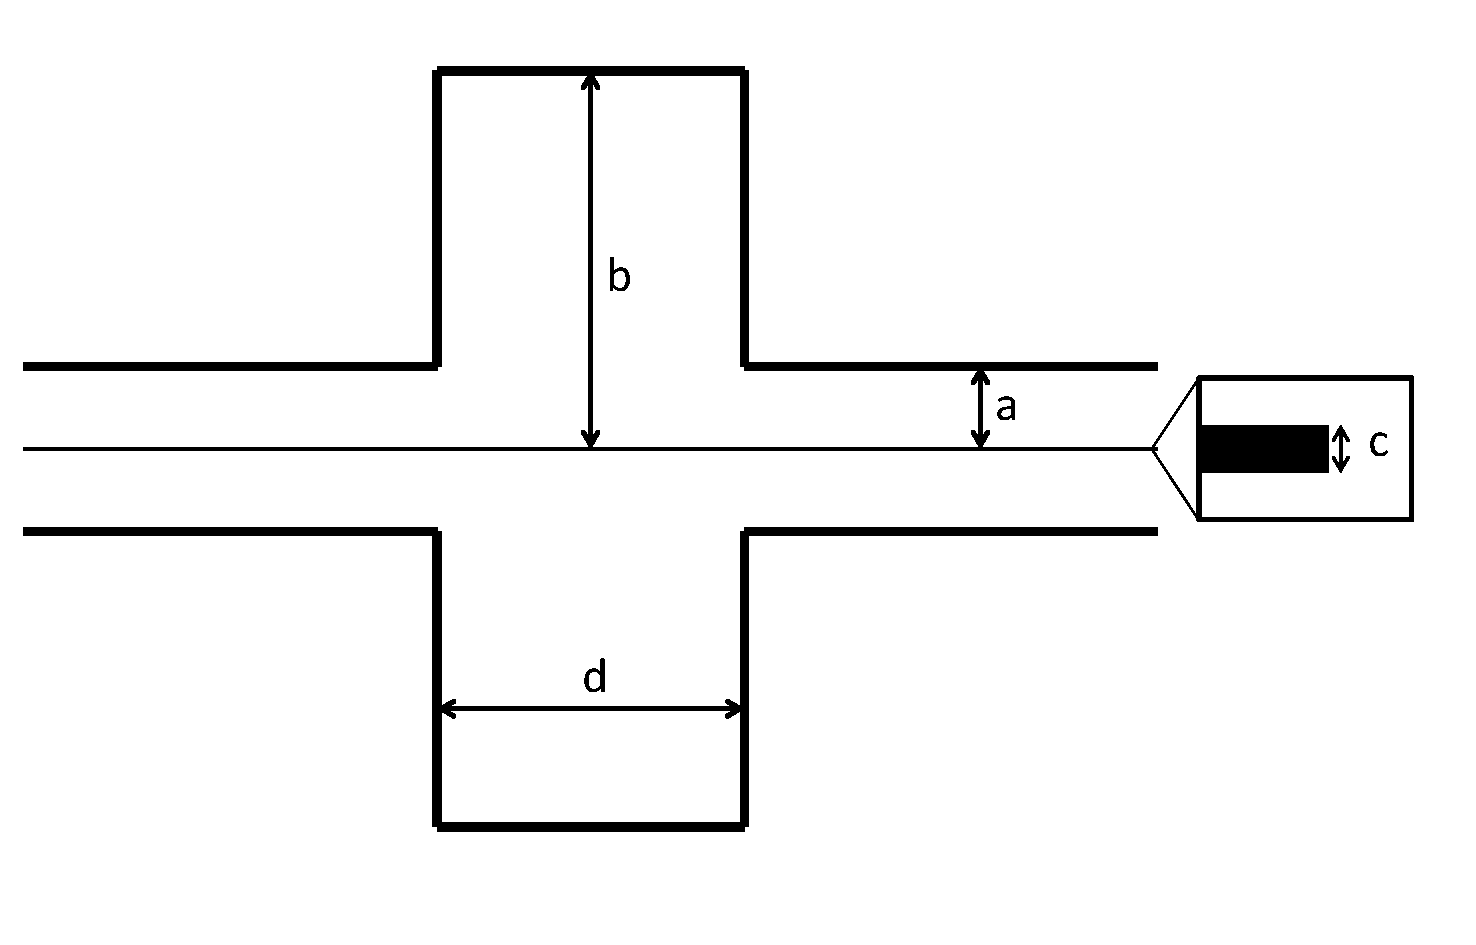
\includegraphics[width=0.625\linewidth]{figures/cavity_beampipe_coaxial.pdf}
\label{fig:cavity_beampipe_coaxial}
}
\caption{Comparison of the geometries of a cavity and attached beampipes \ref{fig:cavity_beampipe} without and \ref{fig:cavity_beampipe_coaxial} with the coaxial wire in place. Note the dimensions and that the dashed line in \ref{fig:cavity_beampipe} represents the rotational plane of symmetry}

\end{figure}

%
%  Things to do for high Q factor measurements
% - Simulation of transmission coefficients with and without coaxial wire
% - Comparison of impedance due to these resonances with time domain simulations
%
%
%
%
%
%
%
%
%
%
